\subsection{Counting Sort}

\subsubsection{Ý tưởng}

Counting Sort không so sánh các phần tử mà dựa trên việc đếm số lần xuất hiện của từng giá trị. Thuật toán tạo một mảng đếm (counting array) để lưu số lần xuất hiện của các giá trị và sử dụng mảng này để xây dựng mảng đã sắp xếp. \cite[p.~102]{hoang2008}

\subsubsection{Mã giả}

\begin{algorithm}[H]
    \caption{Counting Sort \cite[p.~209]{cormen2022} \cite{code-counting}}
    \label{counting-sort}
    
    \SetKwFunction{CountingSort}{CountingSort}
    \SetKwProg{Fn}{procedure}{:}{}
    \Fn{\CountingSort{a\KwSty{[ ]}, n}}{
        $maxVal \gets \max(a)$ \tcp*{Tìm giá trị lớn nhất}
        $minVal \gets \min(a)$ \tcp*{Tìm giá trị nhỏ nhất}
        $range \gets maxVal - minVal + 1$ \tcp*{Phạm vi giá trị trong mảng}
        
        $count[range] \gets \{0\}$ \tcp*{Mảng đếm có kích thước bằng phạm vi giá trị}
        $output[n] \gets \{0\}$ \tcp*{Mảng kết quả}
        
        \For{$i \gets 0$ \KwTo $n-1$}{ 
            $count[a[i] - minVal]++$ \tcp*{Đếm số lần xuất hiện của mỗi phần tử}
        }
        
        \For{$i \gets 1$ \KwTo $range-1$}{
            $count[i] += count[i-1]$ \tcp*{Tính tổng tích lũy}
        }
        
        \For{$i \gets n-1$ \KwSty{downto} $0$}{
            $output[count[a[i] - minVal] - 1] = a[i]$ \tcp*{Xây dựng mảng kết quả} 
            $count[a[i] - minVal]--$
        }
        
        \For{$i \gets 0$ \KwTo $n-1$}{
            $a[i] = output[i]$ \tcp*{Sao chép mảng kết quả vào mảng ban đầu}
        }
    }
\end{algorithm}

\subsubsection{Ví dụ}

Giả sử ta có mảng ban đầu với $n=7$ như sau:
\begin{center}
    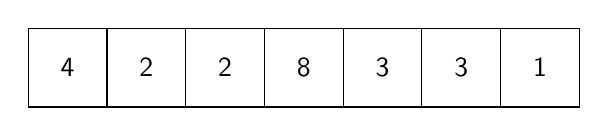
\begin{tikzpicture}[node distance=0cm, font=\sffamily, every node/.style={minimum width=1cm, minimum height=1cm, outer sep=0pt, anchor = west}, line join=miter, line cap=rect]
        \node[draw, fill=white] at (1, 0) {4};
        \node[draw, fill=white] at (2, 0) {2};
        \node[draw, fill=white] at (3, 0) {2};
        \node[draw, fill=white] at (4, 0) {8};
        \node[draw, fill=white] at (5, 0) {3};
        \node[draw, fill=white] at (6, 0) {3};
        \node[draw, fill=white] at (7, 0) {1};
    \end{tikzpicture}
\end{center}

\textbf{Bước 1:} Tìm $min$ và $max$ trong mảng để tính $k = max - min + 1
= 8 - 1 + 1 = 8$. Khởi tạo mảng đếm $count$ có kích thước $k$:

\begin{center}
    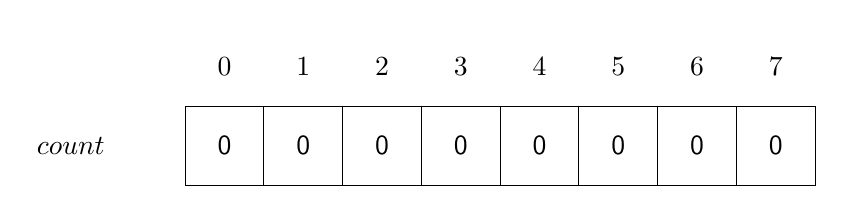
\begin{tikzpicture}[node distance=0cm, font=\sffamily, every node/.style={minimum width=1cm, minimum height=1cm, outer sep=0pt, anchor = west}, line join=miter, line cap=rect]
        \node[font=\rmfamily] at (2, 0) {0};
        \node[font=\rmfamily] at (3, 0) {1};
        \node[font=\rmfamily] at (4, 0) {2};
        \node[font=\rmfamily] at (5, 0) {3};
        \node[font=\rmfamily] at (6, 0) {4};
        \node[font=\rmfamily] at (7, 0) {5};
        \node[font=\rmfamily] at (8, 0) {6};
        \node[font=\rmfamily] at (9, 0) {7};
		\node[font=\rmfamily] at (0, -1) {$count$};
        \node[draw, fill=white] at (2, -1) {0};
        \node[draw, fill=white] at (3, -1) {0};
        \node[draw, fill=white] at (4, -1) {0};
        \node[draw, fill=white] at (5, -1) {0};
        \node[draw, fill=white] at (6, -1) {0};
        \node[draw, fill=white] at (7, -1) {0};
        \node[draw, fill=white] at (8, -1) {0};
        \node[draw, fill=white] at (9, -1) {0};
    \end{tikzpicture}
\end{center}

\textbf{Bước 2:} Duyệt qua từng phần tử trong mảng để đếm số lần xuất hiện
và lưu vào mảng đếm $(count)$ tại vị trí tương ứng với giá trị của phần tử 
đó trừ đi giá trị nhỏ nhất trong mảng đầu vào. Khi đó sẽ thu được mảng:

\begin{center}
    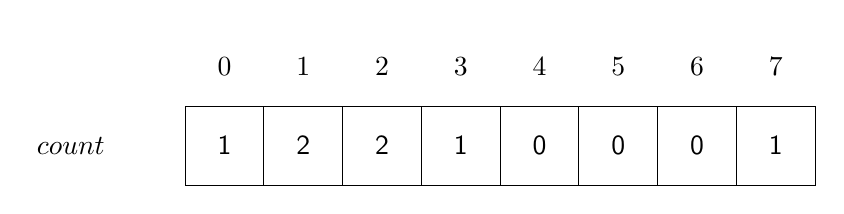
\begin{tikzpicture}[node distance=0cm, font=\sffamily, every node/.style={minimum width=1cm, minimum height=1cm, outer sep=0pt, anchor = west}, line join=miter, line cap=rect]
        \node[font=\rmfamily] at (2, 0) {0};
        \node[font=\rmfamily] at (3, 0) {1};
        \node[font=\rmfamily] at (4, 0) {2};
        \node[font=\rmfamily] at (5, 0) {3};
        \node[font=\rmfamily] at (6, 0) {4};
        \node[font=\rmfamily] at (7, 0) {5};
        \node[font=\rmfamily] at (8, 0) {6};
        \node[font=\rmfamily] at (9, 0) {7};
		\node[font=\rmfamily] at (0, -1) {$count$};
        \node[draw, fill=white] at (2, -1) {1};
        \node[draw, fill=white] at (3, -1) {2};
        \node[draw, fill=white] at (4, -1) {2};
        \node[draw, fill=white] at (5, -1) {1};
        \node[draw, fill=white] at (6, -1) {0};
        \node[draw, fill=white] at (7, -1) {0};
        \node[draw, fill=white] at (8, -1) {0};
        \node[draw, fill=white] at (9, -1) {1};
    \end{tikzpicture}
\end{center}

\textbf{Bước 3:} Tính tổng tích lũy cho mảng đếm $(count)$ sẽ thu được mảng sau:

\begin{center}
    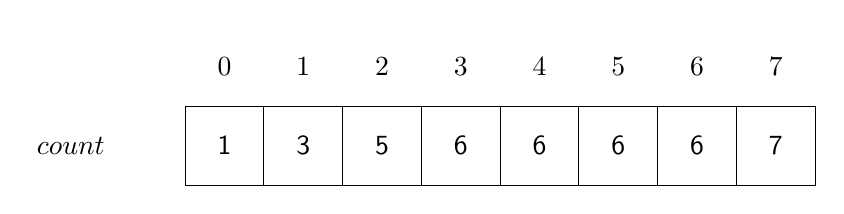
\begin{tikzpicture}[node distance=0cm, font=\sffamily, every node/.style={minimum width=1cm, minimum height=1cm, outer sep=0pt, anchor = west}, line join=miter, line cap=rect]
        \node[font=\rmfamily] at (2, 0) {0};
        \node[font=\rmfamily] at (3, 0) {1};
        \node[font=\rmfamily] at (4, 0) {2};
        \node[font=\rmfamily] at (5, 0) {3};
        \node[font=\rmfamily] at (6, 0) {4};
        \node[font=\rmfamily] at (7, 0) {5};
        \node[font=\rmfamily] at (8, 0) {6};
        \node[font=\rmfamily] at (9, 0) {7};
		\node[font=\rmfamily] at (0, -1) {$count$};
        \node[draw, fill=white] at (2, -1) {1};
        \node[draw, fill=white] at (3, -1) {3};
        \node[draw, fill=white] at (4, -1) {5};
        \node[draw, fill=white] at (5, -1) {6};
        \node[draw, fill=white] at (6, -1) {6};
        \node[draw, fill=white] at (7, -1) {6};
        \node[draw, fill=white] at (8, -1) {6};
        \node[draw, fill=white] at (9, -1) {7};
    \end{tikzpicture}
\end{center}

\textbf{Bước 4:} Xây dựng mảng kết quả theo công thức 
$output[count[input[i] - min] - 1] = input[i]$ và giảm giá trị mảng đếm
tại vị trí vừa truy cập. Khi đó ta được mảng đã sắp xếp:

\begin{center}
    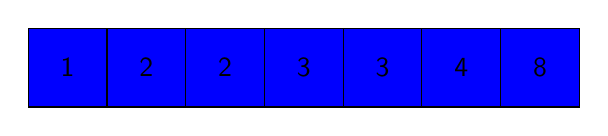
\begin{tikzpicture}[node distance=0cm, font=\sffamily, every node/.style={minimum width=1cm, minimum height=1cm, outer sep=0pt, anchor = west}, line join=miter, line cap=rect]
        \node[draw, fill=blue] at (1, 0) {1};
        \node[draw, fill=blue] at (2, 0) {2};
        \node[draw, fill=blue] at (3, 0) {2};
        \node[draw, fill=blue] at (4, 0) {3};
        \node[draw, fill=blue] at (5, 0) {3};
        \node[draw, fill=blue] at (6, 0) {4};
        \node[draw, fill=blue] at (7, 0) {8};
    \end{tikzpicture}
\end{center}

\subsubsection{Độ phức tạp thuật toán}

Với $k$ là giá trị lớn nhất trong mảng trừ giá trị nhỏ nhất cộng thêm 1. Ta có:

\begin{itemize}
	\item Độ phức tạp thời gian \cite[p.~209]{cormen2022}
	\begin{itemize}[label=$\circ$]
		\item Trường hợp tốt nhất: $O\left(n+k\right)$. Khi khi $k$ nhỏ 
		(các giá trị trong mảng nằm trong một khoảng hẹp), Counting Sort 
		chỉ cần thực hiện một số ít phép đếm và truy cập mảng đếm.
		\item Trường hợp xấu nhất: $O\left(n+k\right)$. Khi $k$ lớn (các 
		giá trị trong mảng nằm trong một khoảng rất rộng), thuật toán 
		vẫn phải tạo và xử lý mảng đếm có kích thước $k$.
		\item Trường hợp trung bình: $O\left(n+k\right)$. Trong mọi 
		trường hợp, Counting Sort luôn thực hiện một số bước cố định: 
		đếm số lần xuất hiện, tính tổng tích lũy và xây dựng mảng kết quả. 
		Do đó, độ phức tạp trung bình cũng là $O\left(n+k\right)$. 
	\end{itemize}
	\item Độ phức tạp không gian: $O\left(n+k\right)$. Counting Sort 
	yêu cầu thêm không gian để lưu trữ:
	\begin{itemize}[label=$\circ$]
		\item Mảng đếm: Có kích thước $k$ để đếm số lần xuất hiện của 
		các giá trị trong mảng đầu vào.
		\item Mảng kết quả: Có kích thước $n$ để lưu trữ mảng đã sắp xếp.
	\end{itemize}
\end{itemize}